\section{The 1-D Ising Model, Continued}
Recall we were studying the 1D Ising Hamiltonian:
\begin{equation}
    H = -\sum_{n=1}^{N-1}J\sigma_n \sigma_{n+1} - B \sum_{n=1}^N \sigma_n.
\end{equation}
This is one of the few exactly solvable cases with a nonzero external $B$ field. All of the other famous solvable Ising models have the $B$-fields turned off. Note that solving the 1-D case is really easy (left as an exercise) if $B = 0$. With $B \neq 0$, we use a transfer matrix technique that we finish today.

Last class we also studied the phase diagram of the Ising model; we considered the boundaries of the phase diagram, though the central areas were left undetermined. In 1D the center of this phase diagram is not very interesting at all (and no interesting phase transition is really observed) but it is still valuable to consider to get used to the model and to explore the analytical techniques to solve it.

\subsection{Large-field case}

Note that in the case where $B \gg J$, the partition function is very simple as we can neglect the exchange/$J$ term in the energy:
\begin{equation}
    Z = \sum_{\sigma_n} \prod_n e^{\frac{B}{k_B T}\sigma_n} = \left(2\cosh\frac{B}{k_B T}\right)^N
\end{equation}
so:
\begin{equation}
    F = -k_B T \ln Z = -k_B T N \ln (2\cosh\frac{B}{k_B T})
\end{equation}
with magnetization per spin:
\begin{equation}
    m = \frac{M}{N} =  \frac{\left.-\dpd{F}{B}\right|_{N, T}}{N} = \tanh(\frac{B}{k_B T})
\end{equation}
which is $\pm 1$ (i.e. full magnetization upwards/downwards) as $B \to \pm \infty$. 

\subsection{The Transfer Matrix and Solving 1-D Ising Model}
We recall we found the transfer matrix:
\begin{equation}
    T_{ab} = \m{e^{\frac{J + B}{k_B T}} & e^{-\frac{J}{k_B T}} \\ e^{-\frac{J}{k_B T}} & e^{\frac{J + B}{k_B T}}}
\end{equation}
and with this we were able to express the partition function for the (general) 1-D Ising model partition function as:
\begin{equation}
    Z = \m{e^{\frac{B}{2k_B T}} & e^{-\frac{B}{2k_B T}}} T^{N - 1}\m{e^{\frac{B}{2k_B T}} \\ e^{-\frac{B}{2k_B T}}}
\end{equation}
we used open boundary conditions here; but it would also be possible to fix the orientations of spins at the edges of the chain, or to use periodic boundary conditions where we identify the first and last spin of the chain. In the limit of large $N$, the boundary conditions are not relevant and the boundary conditions do not matter.


So how do we go about analyzing this partition function? Well, $T_{ab}$ is a real symmetric matrix. A real symmetric matrix can be diagonalized via a similarity transformation:
\begin{equation}
    T = R\Lambda R^T = \m{\cos\theta & -\sin\theta \\ \sin\theta & \cos\theta}\m{t_+ & 0 \\ 0 & t_-}\m{\cos\theta & \sin\theta \\ -\sin\theta & \cos\theta}
\end{equation}
Then, since $RR^T = \mathbb{I}$ it follows that:
\begin{equation}
    T^{N-1} =  \m{\cos\theta & -\sin\theta \\ \sin\theta & \cos\theta}\m{t_+^{N-1} & 0 \\ 0 & t_-^{N-1}}\m{\cos\theta & \sin\theta \\ -\sin\theta & \cos\theta}
\end{equation}
Now we study this when $N$ is large; then the partition function is dominated by the larger eigenvalue $t_+$; we can keep terms of $O(N)$ and throw away terms of $O(1)$. We thus come to the conclusion:
\begin{equation}
    F = -k_B T N\ln t_+.
\end{equation}
Now if we wanted to find this free energy explicitly and confirm this assertion that the larger eigenvalue dominates, we could also explicitly solve this system. For this, the periodic boundary conditions may be easiest, as we can just take the trace of $T^{N-1}$ (and we don't get any boundary terms).

Solving for the eigenvalues of $T$, we find:
\begin{equation}
    t_\pm = e^{\frac{J}{k_B T}}\cosh\frac{B}{k_B T} \pm \sqrt{e^{\frac{2J}{k_B T}}\sinh^2\frac{B}{k_B T} + e^{-\frac{-2J}{k_B T}}}
\end{equation}
which we note are both real and positive. The free energy is then:
\begin{equation}
    F = -k_B T\ln t_+^N = -N J - k_B T N\ln\left[\cosh\frac{B}{k_B T} + \sqrt{\sinh^2\frac{B}{k_B T} + e^{-\frac{4J}{k_B T}}}\right]
\end{equation}
here $-NJ$ is very much like a ``zero point energy''. If we look at the limits of this expression, this matches up with the boundaries of the phase diagram that we analyzed previously! (we can find the magnetization $M = \left.\pd{F}{B}\right|_{N, T}$ and then see that it reproduces our predictions in the $T \to 0/\infty$ and $B \to \pm \infty$ limits). We also note that $F$ is completely non-singular in the inside of the phase diagram, and with the exception at $F = 0, B = 0$ it is also completely non-singular on the boundaries of the phase diagram.

At that point, we cannot use symmetry to conclude that the magnetization is $M = 0$; instead it is history dependent. It is highly ambiguous, and the symmetry is spontaneously broken there.

\subsection{Correlation Functions}
So, we've solved for the thermodynamics of the system! But another line of interest in studying spin systems are correlation functions.

To start, consider $\avg{\sigma_x}$ (one-point correlation function). If we have periodic BCs, then this is site independent and furthermore just gives the magnetization per spin and so:
\begin{equation}
    \avg{\sigma_x} = m
\end{equation}
but if there are other BCs, then we need to take into account corrections:
\begin{equation}
    \avg{\sigma_x} = m + \text{boundary corrections}
\end{equation}
we can explicitly evaluate $\avg{\sigma_x}$ are using the transfer matrix formalism. E.g. for the case of open boundary conditions:
\begin{equation}
    \avg{\sigma_x} = \frac{\m{e^{\frac{B}{2k_B T}} & e^{-\frac{B}{2k_B T}}} T^{x-1} \m{1 & 0 \\ 0 & -1} T^{N - x} \m{e^{\frac{B}{2k_ B T}} \\ e^{-\frac{B}{2k_B T}}}}{Z}
\end{equation}
Now in principle we could evaluate this. We skip this as this is not particularly illuminating. With periodic BCs, we get rid of the boundary terms and just take the trace:
\begin{equation}
    m = \frac{\Tr\left[ T^{x-1} \m{1 & 0 \\ 0 & -1} T^{N - x}\right]}{\Tr T^{N-1}} = \frac{\Tr\left[ T^{N-1} \m{1 & 0 \\ 0 & -1}\right]}{\Tr T^{N-1}} = \frac{c_+t_+^{N-1} - c_-t_-^{N-1}}{c_+t_+^{N-1} + c_-t_-^{N-1}}
\end{equation}
where we have used the cyclicity of the Trace; $\Tr(ABC) = \Tr(CAB) = \Tr(BCA)$. 

There are then higher-point correlation functions. We consider the two-point correlation function (which already give us some interesting information):
\begin{equation}
    \avg{\sigma_x \sigma_y}
\end{equation}
but actually the connected correlation function will be a little more interesting to study:
\begin{equation}
    \avg{\sigma_x \sigma_y} - \avg{\sigma_x}\avg{\sigma_y}
\end{equation}
this in principle again we can evaluate for any boundary condition, but again let's just look at the simplest case of the periodic BCs. Then:
\begin{equation}
    \avg{\sigma_x\sigma_y} = \frac{\Tr\left[T^{x-1}\pauliz T^{y-x} \pauliz T^{N-y}\right]}{\Tr T^{N-1}}
\end{equation}
and $\avg{\sigma_x}$ is independent of $x$/the site, so $\avg{\sigma_x}\avg{\sigma_y} = \avg{\sigma_x}^2$ and so:
\begin{equation}
    \avg{\sigma_x \sigma_y} - \avg{\sigma_x}\avg{\sigma_y} = \frac{\Tr\left[T^{x-1}\pauliz T^{y-x} \pauliz T^{N-y}\right]}{\Tr T^{N-1}} -  \left(\frac{\Tr\left[ T^{x-1} \m{1 & 0 \\ 0 & -1} T^{N - x}\right]}{\Tr T^{N-1}}\right)^{2}
\end{equation}

Now we can plug in the diagonal form of $T$ and evaluate all of this; at the end of the day\footnote{I take home my hard earned pay all alone\ldots} we end up with:

\begin{equation}
    \avg{\sigma_x \sigma_y} - \avg{\sigma_x}\avg{\sigma_y} = \frac{t_+^{y-x}t_-^{N-1-(y-x)} + t_-^{y-x}t_+^{N-1-(y-x)}}{t_+^{N-1} + t_-^{N-1}}
\end{equation}
Now we notice a symmetry; the connected correlation function only depends on the distance from $y$ to $x$, but not the actual sites themselves! Now, if we assume that the sites $y, x$ are sufficiently close, i.e. we work in the limit:
\begin{equation}
    N \gg (y - x) \geq 1
\end{equation}
the above simplifies to:
\begin{equation}
    \avg{\sigma_x \sigma_y} - \avg{\sigma_x}\avg{\sigma_y} \approx \left(\frac{t_-}{t_+}\right)^{y-x} = e^{-\abs{x-y}/\xi}
\end{equation}
where $\xi$ is the \emph{correlation length}. To get this correlation length, we can take a logarithm of both sides:
\begin{equation}
    \xi = \frac{1}{\ln(t_+/t_-)}
\end{equation}
which we can then find explicitly by plugging in the form of the eigenvalues.

\subsection{The 1-D Ising Model is Disordered at Finite Temperature}
Landau gives the following argument for why the Ising model is always disordered in one dimension, that is to say, why is $m = 0$ in 1-D on the $B = 0$ line for all $T> 0$. 

\begin{figure}[htbp]
    \centering
    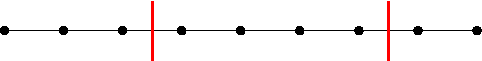
\includegraphics{Images/fig-1DIsingdisorder.pdf}
    \caption{Cartoon of the setup for Landau's argument for disorder in the 1D Ising model. We consider flips in the bonds between spins (domain walls) in the chain of spins.}
    \label{fig-1DIsingdisorder}
\end{figure}

The Hamiltonian is minimized if all spins are aligned. The next lowest energy state is one where there is a single flipped spin. Compared to the lowest energy state, this has energy penalty $-2J$ and so has a boltzmann factor $e^{-2J/k_B T}$ that suppresses the probability of this happening. So up to an overall factor $e^{JN/k_B T}$ which takes into account the zero point energy, the first twoo terms in the partition function (the low-$T$ expansion) is:
\begin{equation}
    Z \sim 1 + Ne^{-2J/k_B T}
\end{equation}
with the $N$ appearing as these are the possible bonds (domain walls) between spins that could be flipped. Then we add the next term for 2 flips, which yields:
\begin{equation}
    Z \sim 1+ Ne^{-2J/k_B T} + \binom{N}{2}e^{-4J/k_B T}
\end{equation}
and in general the term with $n$ flipped bonds has coefficient $\binom{N}{n}$ and so:
\begin{equation}
    Z \sim 1 + Ne^{-2J/k_B T} + \binom{N}{2}e^{-4J/k_B T} + \ldots + \binom{N}{n}e^{-2nJ/k_B T} + \ldots
\end{equation}
now, if we look at the most likely distribution, we see that the $n = N/2$ unmagnetized state is favoured. The entropy grows faster than the number of bonds, vs. the energy grows proportionally than the number of bonds; so the entropy wins out and we see that the unmagnetized state is favoured.

Why does this argument fail in higher dimensions? Because the domain walls scale differently in 2D. The entropy grows as the number of closed paths (rather than as the number of points on the line) which means that the above argument does not apply in the same way (and we do get a phase transition in higher dimensions)!

Lots of cool stuff that Ising models can be tied to... e.g. Majorana fermions in 2D, random surface theories, fermionic string theories in 3D...

\subsection{Teaser - Infinite Range Ising Model}
We look at another analytically solvable Ising model. Here, we remove the restriction that the spins only interact with their nearest neighbours. Specifically, we consider the case where every spin interacts with every other spin with the same interaction strength. While this is not at all a physically realistic system (because interactions are not infinite range in real life, of course) but we will see that the phase diagram of this model is more interesting, with phase transitions occuring at finite $T$ across $B = 0$. 

Our Hamiltonian is:
\begin{equation}
    H = -\frac{J}{N}\sum_{n, n'}\sigma_n \sigma_{n'} - B\sum_n \sigma_n
\end{equation}
where the sum $\sum_{n, n'}$ runs over all pairs of spins in the lattice. We are able to evaluate this by summing over one spin at a time (with each spin giving an equal contribution to the overall partition function), because all spins look the same here:
\begin{equation}
    Z = \sum_{\sigma_n} e^{\frac{J}{k_B T}\sum_{n, n'}\sigma_n \sigma_{n'} + \frac{B}{k_B T}\sum_n \sigma_n}
\end{equation}
This looks awful, but we can consider an analogy with a Gaussian integral. Consider:
\begin{equation}
    \int_{-\infty}^\infty dm e^{-\left(m - \frac{1}{N}\sum_x \sigma_x\right)^2\frac{JN}{k_B T}}
\end{equation}
We can solve this by translating the integral to get rid of $\sum_x \sigma_x$ which is a constant w.r.t. the variable of integration. The integral then evaluates to:
\begin{equation}
    \int_{-\infty}^\infty dm e^{-\left(m - \frac{1}{N}\sum_x \sigma_x\right)^2\frac{JN}{k_B T}} = \sqrt{\frac{k_B T}{NJ}\pi}
\end{equation}
So then:
\begin{equation}
    1 = \sqrt{\frac{NJ}{\pi k_B T}}\int_{-\infty}^\infty dm e^{-\left(m - \frac{1}{N}\sum_x \sigma_x\right)^2\frac{JN}{k_B T}}
\end{equation}
Now let us put this factor of 1 into the partition function. We will then see that terms cancel, and we get an integral that we can solve - if $N$ is large - using a saddle point integration technique. From this we can obtain the free energy and learn the thermodynamic properties of the system.